\chapter{Dibujo de Ingeniería}
El \textbf{Dibujo} es la expresión máxima del ser humano, como dice la frase popular: ``Un dibujo dice más que mil palabras''.
El dibujo también es una representación gráfica de algo real.Es un lenguaje gráfico, ya que usa figuras para comunicar pensamientos e ideas.
Existen tipos de dibujos, se abordarán los cuatro más importantes y de interés:
\begin{itemize}
	\item Dibujo Básico: Letras y letreros, alfabeto y líneas, símbolo de un plano, dibujo geométrico, escalas y elementos básicos
	\item Dibujo de obras hidráulicas: Elementos que lo componen, unidades de trabajo y proyección ortogonal
	\item Dibujo de mecanismos: materiales formas, escalas, perspectivas
	\item Dibujo arquitectónico: Unidades, elementos y la ideología.
\end{itemize}

Es importante hacer el comentario que una herramienta de trabajo serán las hojas, pero existen diferentes tamaños
y formatos, por lo cual, en la figura \ref{fdi1}, se muestran los formatos de papel. En ésta sección,
se usará el tamaño A3 $(297mm \times  420mm)$. Al mismo tiempo que se usarán:

\begin{enumerate}
	\item Lápices de grafito H,2B,2H y HB
	\item Juego de escuadras
	\item Gomas de migajón
	\item Compás de precisión
	\item Estilógrafo
	\item regla con escalas
\end{enumerate}

\begin{figure}

	\centerline{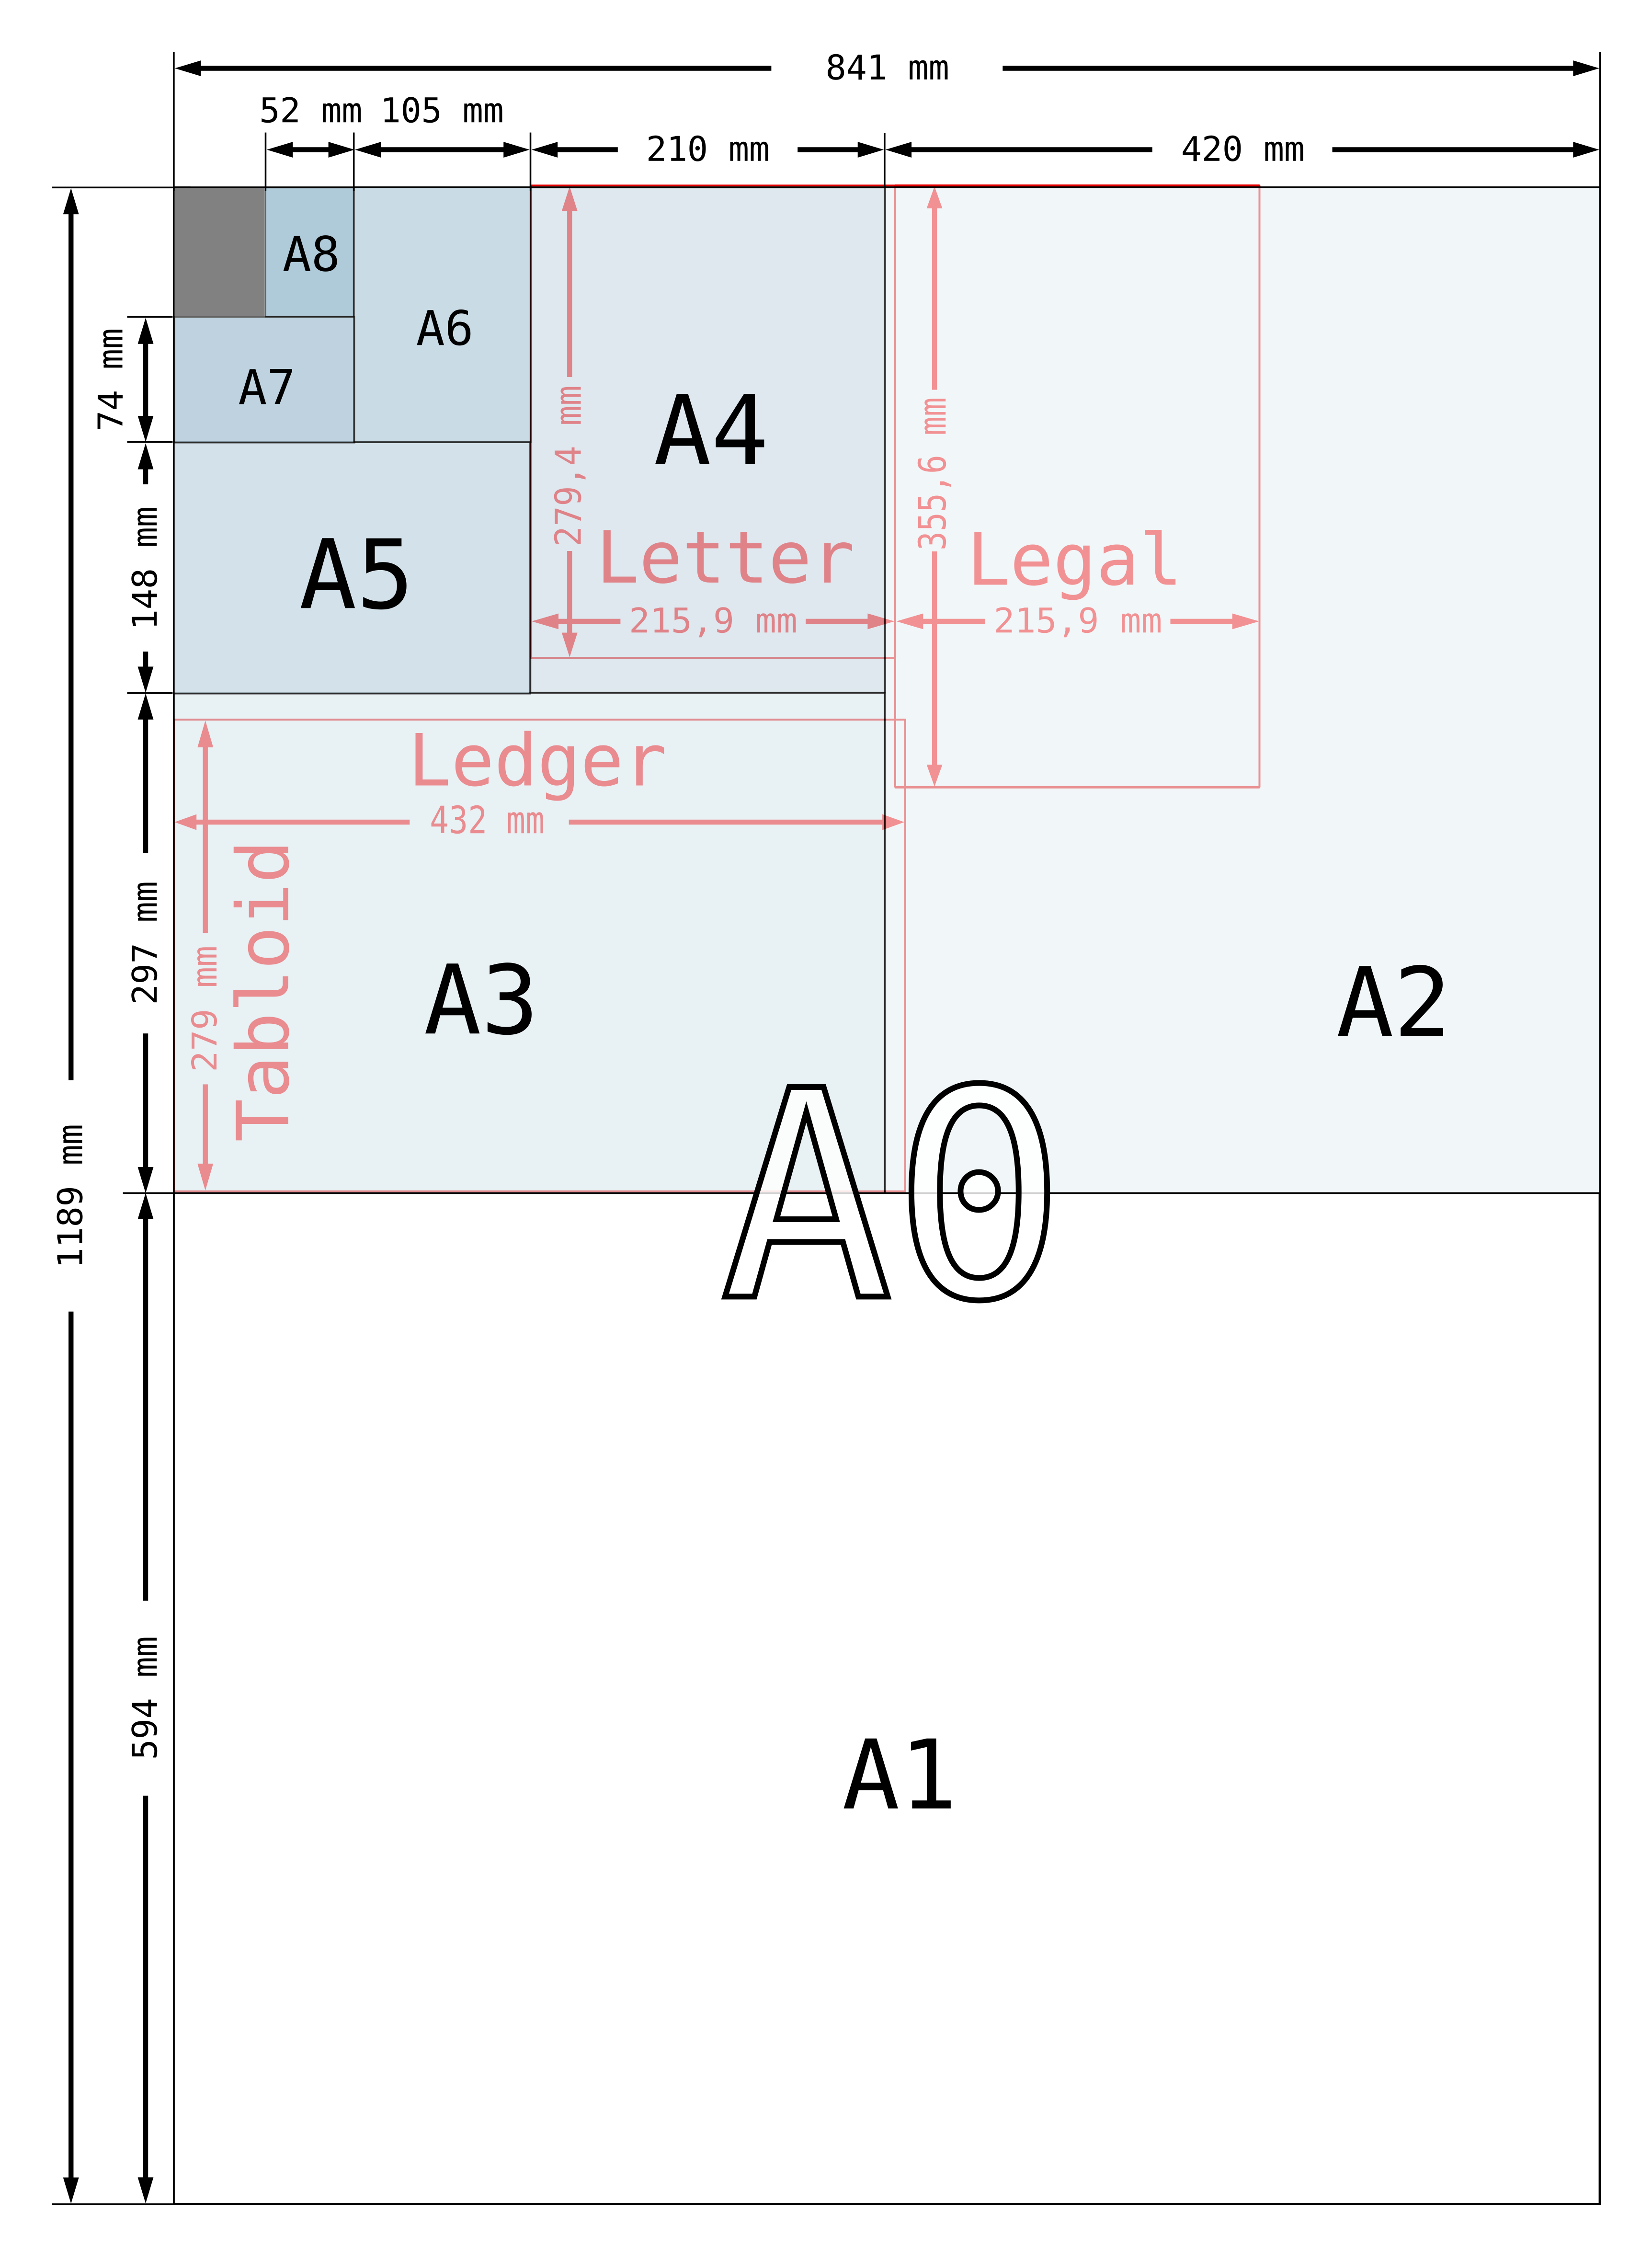
\includegraphics[width=1\textwidth]{fdi1.png}}
	\caption{Comparación entre los formatos ISO (Europeo) y A (Americano)}
	\label{fdi1}
\end{figure}

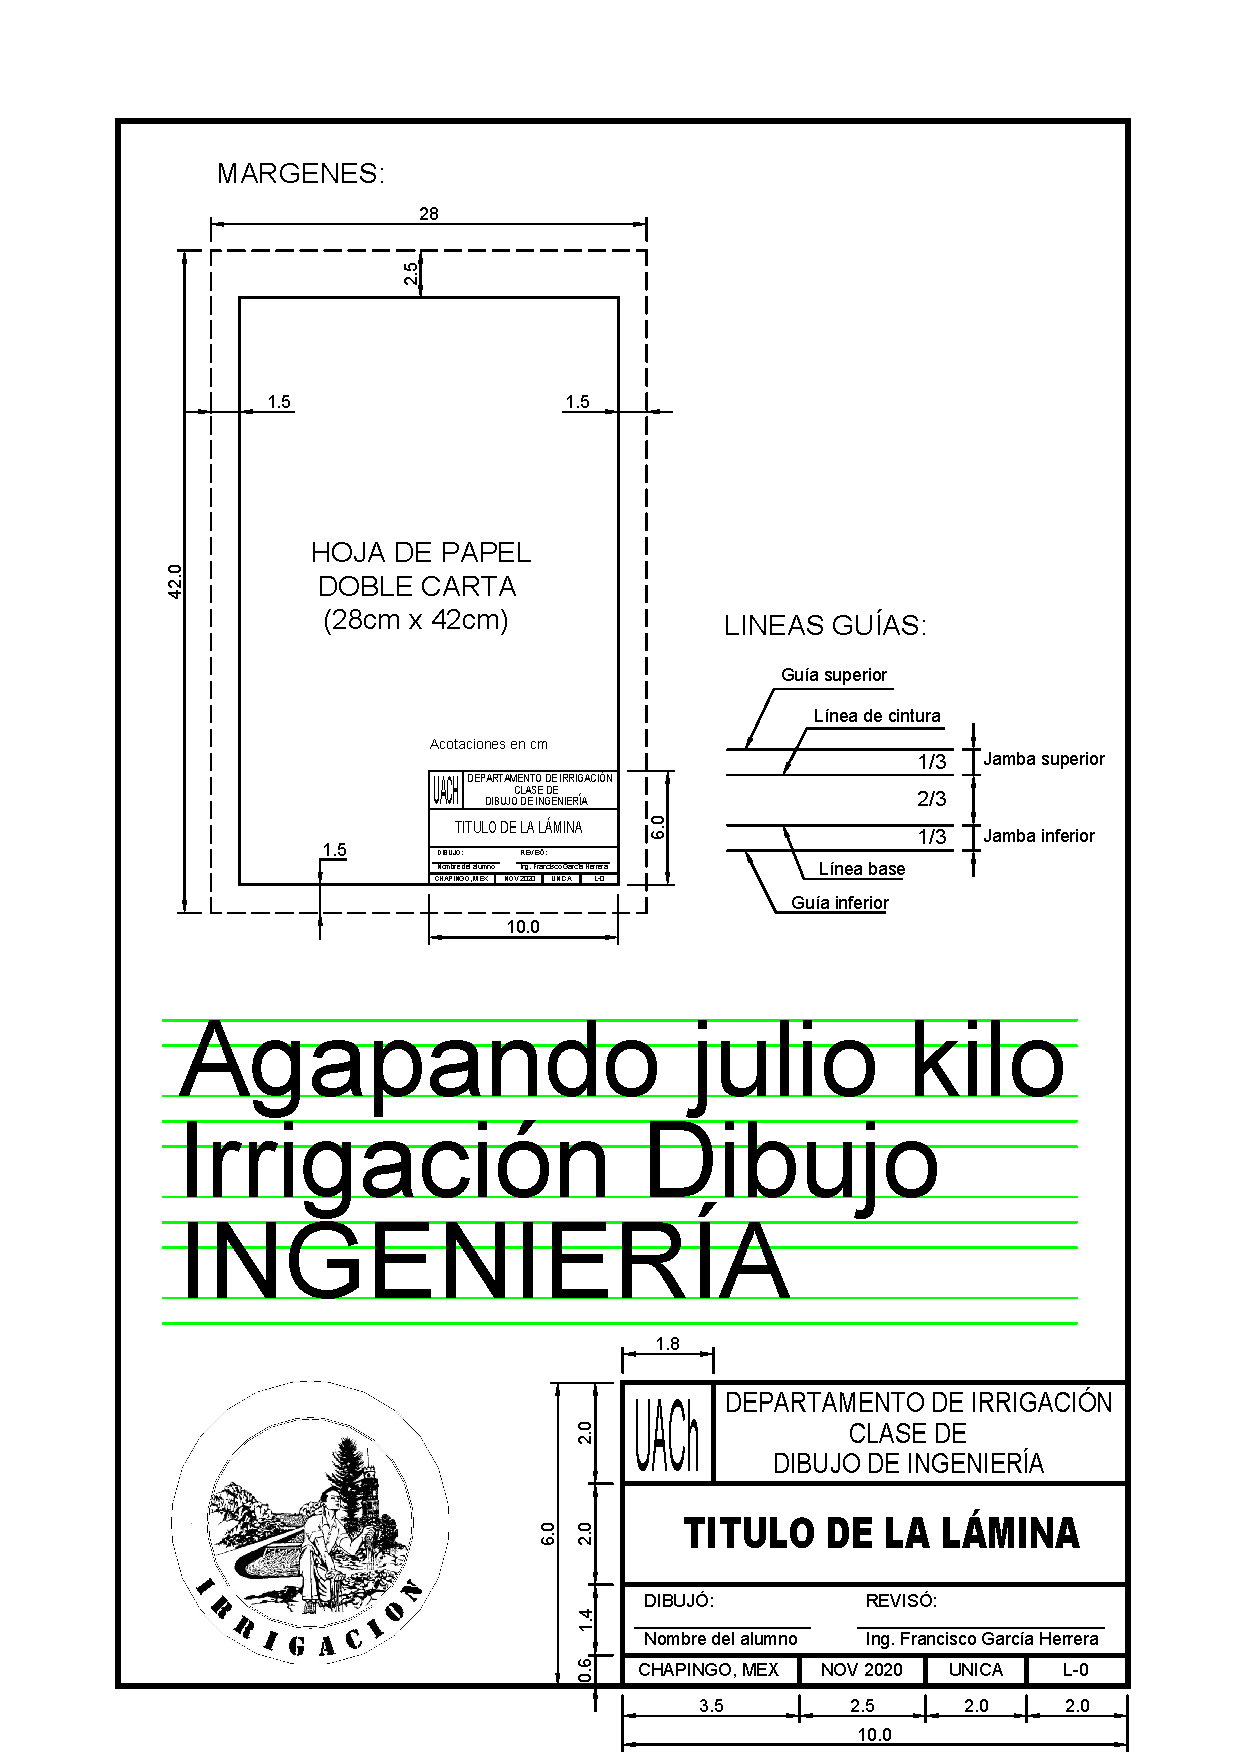
\includepdf[pages=1]{L0_2020.pdf}


El objetivo es que las medidas de sus lados guardan una proporción tal que, dividiéndolo al medio en su longitud, cada una de las mitades
siguen guardando la misma relación entre sus lados que el pliego original.
Para que la medida de los lados cumpla esta propiedad, deben guardar una relación particular. Si se llama $x$ a un lado e $y$ al otro:

\begin{equation*}
	\frac{x}{y} = \frac{y}{\frac{x}{2}} = \frac{2}{\frac{x}{y}} = \left(\frac{x}{y} \right) ^2  = 2\implies \sqrt{2}\simeq 1.4142
\end{equation*}

Sobre los \textbf{membretes}, véase la figura, se concentran los datos más importantes
sobre nuestro dibujo

\begin{figure}
	\centerline{
\includegraphics[width=0.5\textwidth]{fdi2.png}}
	\caption{Ejemplo de un membrete de la UACh, México}
	\label{fdi2}
\end{figure}

Algunas herramientas complementarias son las siguientes:

\begin{itemize}
	\item Regla T
	\item Restirador
	\item Máquina universal
	\item Rapidógrafos
	\item Tinta China
	\item Compás
	\item Escalímetro, regla francesa, curvígrafo
	\item Compás de precisión(brazos rígidos, brazos articulados, de bara, de bombilla, puntas secas)
	\item Plantillas (círculos, elipses)
	\item plotter
	\item Curvímetro, odómetro, planímetro.
\end{itemize}

Se ha comentado sobre las herramientas necesarias para llevar a cabo los dibujos, pero la medición
es el pilar fundamental.

Se ha comentado sobre las herramientas necesarias para llevar a cabo los dibujos, pero la medición
es el pilar fundamental. Existen ciertas reglas para representar las unidades:

\begin{enumerate}
	\item Las enumeraciones se escriben en minúsculas
	\item se escriben en singular
\end{enumerate}

\section{Precauciones en el dibujo}
\begin{enumerate}
	\item Nunca se principie un trabajo sin limpiar previamente el ``restirador'' y los
	      instrumentos de dibujo.
	\item Nunca se trabaje con el ``restirador'' obstruido por una serie de instrumentos
	      o equipo innecesario.
	\item Nunca se corte el papel con una cuchilla usando la regla T o las escuadras
	      como guías.
	\item Nunca se dejen destapadas las botellas de tinta china.
	\item Nunca se cargue con tinta china la plumilla o el estilógrafo sobre el dibujo.
	\item Nunca se use tinta china distinta de la que tiene el instrumento de dibujo.
	\item Nunca se utilice el escalímetro para trazar líneas.
\end{enumerate}

Tenemos las siguientes unidades de medición:

\begin{multicols*}{2}
	\textbf{Longitud:}
	\begin{enumerate}
		\item kilómetro $(km)$
		\item Metro $(m)$
		\item Decímetro $(dm)$
		\item Centímetro $(cm)$
		\item Milímetro $(mm)$
		\item Pie $(pie, ft)$
		\item Pulgada $(pulg, in)$
	\end{enumerate}

	\textbf{Superficie:}
	\begin{enumerate}
		\item Hectárea $(ha)$
		\item Kilómetro cuadrado $(km^2 )$
		\item Metro cuadrado $(m^2 )$
		\item Decímetro cuadrado $(dm^2 )$
		\item Centímetro cuadrado $(cm^2 )$
		\item Milímetro cuadrado $(mm^2 )$
		\item pie cuadrado $(pie^2 ,ft^2 )$
		\item Pulgada cuadrada $(pulg^2 , in^2 )$
	\end{enumerate}

	\textbf{Peso lineal:}
	\begin{enumerate}
		\item Tonelada por metro $\left(\frac{t}{m}\right) $
		\item kilómetro por metro $\left(\frac{kg}{m}\right) $
		\item Kilogramo por centímetro $\left(\frac{lb}{ft}\right) $
		\item libra pie $\left(\frac{lb}{pulg}\right) $
	\end{enumerate}

	\textbf{Trabajo:}
	\begin{enumerate}
		\item Tonelada por metro $ \left(t\cdot m \right)$
		\item Kilogramo por metro $\left(kg \cdot m\right) $
		\item Kilogramo por centímetro $\left(kg \cdot cm\right) $
		\item Libra pie $\left(lb \cdot pie \right) $
	\end{enumerate}

	\textbf{Tiempo:}
	\begin{enumerate}
		\item Hora $\left( hr \right) $
		\item Minuto $\left( min \right)$
		\item Segundo $\left( s \right) $
	\end{enumerate}

	\textbf{volumen:}
	\begin{enumerate}
		\item Metro cúbico $(m^3)$
		\item decímetro cúbico $(dm^3)$
		\item centímetro cúbico $(cm^3)$
		\item Litro $\left( l \right) $
		\item Pie cúbico  $(pie^3,ft^3)$
		\item Pulgada cúbica $(pulg^3, in^3)$
	\end{enumerate}

	\textbf{Peso:}
	\begin{enumerate}
		\item Tonelada métrica $(t)$
		\item Kilogramo $(kg)$
		\item Gramo $(g)$
		\item Libra $(lb)$
	\end{enumerate}

	\textbf{Presión:}
	\begin{enumerate}
		\item Tonelada por metro cuadrado $\left(\frac{t}{m^2 }\right) $
		\item Kilogramos por metro cuadrado $\left(\frac{kg}{m^2 }\right) $
		\item Kilogramos por centímetro cuadrado $\left(\frac{kg}{m^2 }\right) $
		\item Libra por pie cuadrado $\left(\frac{lb}{ft^2 }\right) $
		\item Libra por pulgada cuadrada $\left(\frac{lb}{pulg^2 }\right) $
	\end{enumerate}

	\textbf{Gasto:}
	\begin{enumerate}
		\item Metros cúbicos por segundo $\left(\frac{m^3}{s}\right) $
		\item Litros por segundo $\left(\frac{l}{s}\right)$
		\item Pies cúbicos por segundo $\left(\frac{pie^3}{s}\right) $
		\item Galones por minuto $\left(\frac{gal}{min}\right) $
	\end{enumerate}

	\textbf{Velocidad:}
	\begin{enumerate}
		\item Metro por segundo $\left(\frac{m}{s}\right) $
		\item Kilómetro por hora $\left(\frac{km}{h}\right) $
		\item Pie por segundo $\left(\frac{ft}{s}\right) $
	\end{enumerate}
\end{multicols*}


\section{Líneas para los dibujos}
\begin{definition}[Plano]
	Es la representación a escala de un objeto. Si el dibujo no está a escala, se denomina croquis
\end{definition}
\begin{enumerate}
	\item Línea de perímetros: Utilizada para el contorno o perímetro de una línea de objetos. Espesor de la línea de acuerdo con el tamaño y escala de dibujo. Mismo espesor para todas las partes del dibujo trazadas a la misma escala.
	      \begin{center}
		      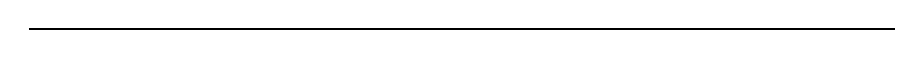
\begin{tikzpicture}
			      \draw[thick] (0,0) -- (11,0);
		      \end{tikzpicture}
	      \end{center}
	\item Línea de construcción invisible: Utilizada para indicar detalles ocultos. Con el espesor especificado en el número uno. Rasgos de 3mm de longitud y espacios de 1mm.
	      \begin{center}
		      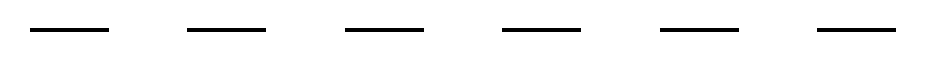
\begin{tikzpicture}
			      \draw[ultra thick] (0,0) -- (1,0);
			      \draw[ultra thick] (2,0) -- (3,0);
			      \draw[ultra thick] (4,0) -- (5,0);
			      \draw[ultra thick] (6,0) -- (7,0);
			      \draw[ultra thick] (8,0) -- (9,0);
			      \draw[ultra thick] (10,0) -- (11,0);
		      \end{tikzpicture}
	      \end{center}
	\item Acotaciones: Se utiliza para denotar una magnitud en el dibujo, espesor menor que el indicado en el No. 1, suficientemente gruesa para obtener una buena copia xerox.
	      \begin{center}
		      \begin{tikzpicture}
			      \draw[<->] (0,0) -- (11,0);
		      \end{tikzpicture}
	      \end{center}

	\item Línea de eje o línea de centro: Utilizada para indicar simetría en el dibujo o el eje del centro de un círculo. Espesor indicado en el No. 3.
	      \begin{center}
		      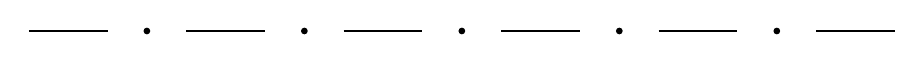
\begin{tikzpicture}
			      \draw[thick] (0,0) -- (1,0);
			      \filldraw [black] (1.5,0) circle (1pt);
			      \draw[thick] (2,0) -- (3,0);
			      \filldraw [black] (3.5,0) circle (1pt);
			      \draw[thick] (4,0) -- (5,0);
			      \filldraw [black] (5.5,0) circle (1pt);
			      \draw[thick] (6,0) -- (7,0);
			      \filldraw [black] (7.5,0) circle (1pt);
			      \draw[thick] (8,0) -- (9,0);
			      \filldraw [black] (9.5,0) circle (1pt);
			      \draw[thick] (10,0) -- (11,0);
		      \end{tikzpicture}
	      \end{center}

	\item De referencia: Son líneas de guía para la construcción del dibujo. Espesor del No.3. o menor.
	      \begin{center}
		      \begin{tikzpicture}
			      \draw (0,0) -- (11,0);
		      \end{tikzpicture}
	      \end{center}
	\item Trazas del plano de corte: Utilizadas para indicar cortes en el dibujo. Espesor 1.6 veces el indicado en el No.1. Las flechas señalan la dirección y el sentido de las visuales. Para referirse a este corte cítese las letras (A-A) que se dibujan junto a las flechas.
	      \begin{center}
		      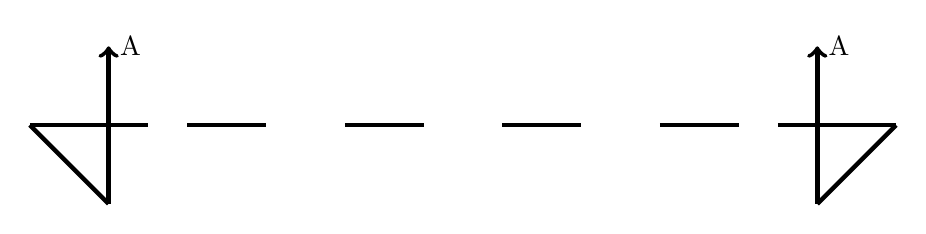
\begin{tikzpicture}
			      \draw[ultra thick] (0,0) -- (1.5,0);
			      \draw[ultra thick] (0,0) -- (1,-1);
			      \draw[ultra thick,->] (1,-1) -- (1,1) node[anchor=west]{A};
			      \draw[ultra thick] (2,0) -- (3,0);
			      \draw[ultra thick] (4,0) -- (5,0);
			      \draw[ultra thick] (6,0) -- (7,0);
			      \draw[ultra thick] (8,0) -- (9,0);
			      \draw[ultra thick] (9.5,0) -- (11,0);
			      \draw[ultra thick] (11,0) -- (10,-1);
			      \draw[ultra thick,->] (10,-1) -- (10,1) node[anchor=west]{A};
		      \end{tikzpicture}
	      \end{center}
	\item Línea para perímetro de cortes: Se utilizan para enmarcar el parea de corte. El espesor 1.6 veces el especificado en el No.1. Este espesor de línea se usará en los dibujos para definir en el corte los perímetros de la estructura.
	      \begin{center}
		      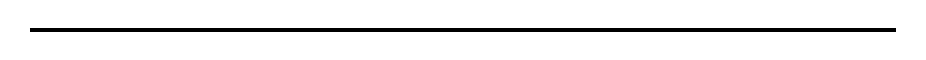
\begin{tikzpicture}
			      \draw[ultra thick] (0,0) -- (11,0);
		      \end{tikzpicture}
	      \end{center}
	\item Líneas de discontinuidad: Se utiliza para dibujar objetos muy largos de la misma forma y dimensiones continuas. Espero un poco menor que el especificado en el No.1.
	      \begin{center}
		      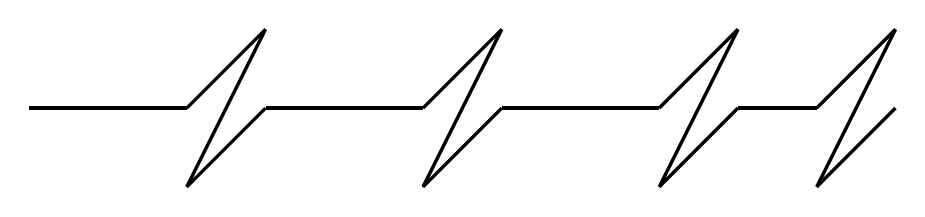
\begin{tikzpicture}
			      \draw[very thick] (0,0) to (2,0);
			      \draw[very thick] (2,0) to (3,1);
			      \draw[very thick] (3,1) to (2,-1);
			      \draw[very thick] (2,-1) to (3,0);

			      \draw[very thick] (3,0) to (5,0);
			      \draw[very thick] (5,0) to (6,1);
			      \draw[very thick] (6,1) to (5,-1);
			      \draw[very thick] (5,-1) to (6,0);

			      \draw[very thick] (6,0) to (8,0);
			      \draw[very thick] (8,0) to (9,1);
			      \draw[very thick] (9,1) to (8,-1);
			      \draw[very thick] (8,-1) to (9,0);

			      \draw[very thick] (9,0) to (10,0);
			      \draw[very thick] (10,0) to (11,1);
			      \draw[very thick] (11,1) to (10,-1);
			      \draw[very thick] (10,-1) to (11,0);
		      \end{tikzpicture}
	      \end{center}
\end{enumerate}

\textbf{Escala gráfica}

La escala gráfica es la representación dibujada en un mapa, carta náutica o un plano con escala unidad por unidad, donde cada segmento muestra la relación entre la longitud de la representación y la de la realidad.
\begin{equation}
	\text{Escala}=\frac{\text{Medida del dibujo}}{\text{Medida real}}
\end{equation}

\subsection{Alfabeto en el plano}
Indicaciones comunes:

\begin{multicols*}{2}
	\begin{enumerate}
		\item Poblaciones
		\item Edificios o casas aisladas
		\item Iglesia
		\item Panteón
		\item Línea de propiedad no cercada
		\item Cerca de alambre de púas
		\item Cerca de suelos vivo o árboles
		\item Cerca de piedras
		\item Carretera pavimentadas
		\item Camino vecinal
		\item Camino de herradura o vereda
		\item Ferrocarril
		\item Línea telefónica o línea telegráfica
		\item Línea de energía eléctrica
		\item Línea divisora Internacional
		\item Lindero de estado
		\item Lindero de municipio
		\item Río
		\item Vaso de almacenamiento o lago
		\item Pantano
		\item Curvas de nivel
		\item Depresión
		\item Línea de vértice de poligonal
		\item Vértice de triangulación
		\item Terraplén
		\item Corte o tajo
		\item Bordo de entarquinamiento
		      %    \item Canal principal
		      %    \item Canal secundario
		      %    \item Presa derivadora
		      %    \item Sidón
		      %    \item Puente canal
		      %    \item Rápida
		      %    \item Caída
	\end{enumerate}
\end{multicols*}

\section{Dibujo de geometría}

La geometría descriptiva tiene como campo de estudio, la axonometría.
A continuación, se mostrarán algunos dibujos con los que puedes generar entes geométricos:

Trazar una perpendicular en un punto:
\begin{center}
	\begin{tikzpicture}[scale=1]
		\tkzSetUpCompass[color=red, line width=1 pt,style=solid]
		\tkzDefPoints{0/0/A, 4/0/B}
		\tkzDrawPoints(A,B)
		\tkzLabelPoint[left](A){$A$}
		\tkzLabelPoint[right](B){$B$}
		\tkzDrawSegment(A,B)
		\tkzInterCC(A,B)(B,A)
		\tkzGetFirstPoint{C}
		\tkzGetSecondPoint{D}
		\tkzCompass[](A,C)
		\tkzCompass[](B,C)
		\tkzCompass[](A,D)
		\tkzCompass[](B,D)
		\tkzDrawPoints[color=black](C,D)
		\tkzLabelPoint[above](C){$C$}
		\tkzLabelPoint[below](D){$D$}
		\tkzDrawSegment(C,D)
		\tkzInterLL(A,B)(C,D)
		\tkzGetPoint{M}
		\tkzDrawPoints[color=blue](M)
		\tkzLabelPoint[color=blue, above right](M){$M$}
	\end{tikzpicture}
\end{center}

Dibujar dos lineas tangentes a dos círculos de diferente radio:

\begin{center}
	\begin{tikzpicture}[scale=.75,rotate=-30]
		\tkzDefPoint(0,0){O}
		\tkzDefPoint(4,-5){A}
		\tkzDefIntSimilitudeCenter(O,3)(A,1)
		\tkzGetPoint{I}
		\tkzExtSimilitudeCenter(O,3)(A,1)
		\tkzGetPoint{J}
		\tkzDefTangent[from with R= I](O,3 cm)
		\tkzGetPoints{D}{E}
		\tkzDefTangent[from with R= I](A,1 cm)
		\tkzGetPoints{D'}{E'}
		\tkzDefTangent[from with R= J](O,3 cm)
		\tkzGetPoints{F}{G}
		\tkzDefTangent[from with R= J](A,1 cm)
		\tkzGetPoints{F'}{G'}
		\tkzDrawCircle[R,fill=red!50,opacity=.3](O,3 cm)
		\tkzDrawCircle[R,fill=blue!50,opacity=.3](A,1 cm)
		\tkzDrawSegments[add = .5 and .5,color=red](D,D' E,E')
		\tkzDrawSegments[add= 0 and 0.25,color=blue](J,F J,G)
		\tkzDrawPoints(O,A,I,J,D,E,F,G,D',E',F',G')
		\tkzLabelPoints[font=\scriptsize](O,A,I,J,D,E,F,G,D',E',F',G')
	\end{tikzpicture}
\end{center}

La intersección $H$ de las tres alturas de un triángulo se llama ortocentro.

\begin{center}
	\begin{tikzpicture}
		\tkzDefPoint(0,0){A}
		\tkzDefPoint(5,1){B}
		\tkzDefPoint(1,4){C}
		\tkzClipPolygon(A,B,C)
		\tkzDefTriangleCenter[ortho](B,C,A)
		\tkzGetPoint{H}
		\tkzDefSpcTriangle[orthic,name=H](A,B,C){a,b,c}
		\tkzDrawPolygon[color=blue](A,B,C)
		\tkzDrawPoints(A,B,C,H)
		\tkzDrawLines[add=0 and 1](A,Ha B,Hb C,Hc)
		\tkzLabelPoint(H){$H$}
		\tkzAutoLabelPoints[center=H](A,B,C)
		\tkzMarkRightAngles(A,Ha,B B,Hb,C C,Hc,A)
	\end{tikzpicture}
\end{center}

Centroide:

\begin{center}
	\begin{tikzpicture}[scale=.75]
		\tkzDefPoints{-1/1/A,5/1/B}
		\tkzDefEquilateral(A,B)
		\tkzGetPoint{C}
		\tkzDefTriangleCenter[centroid](A,B,C)
		\tkzGetPoint{G}
		\tkzDrawPolygon[color=brown](A,B,C)
		\tkzDrawPoints(A,B,C,G)
		\tkzDrawLines[add = 0 and 2/3](A,G B,G C,G)
	\end{tikzpicture}
\end{center}


triangulo inscrito en un circulo

\begin{center}
	\begin{tikzpicture}
		\tkzDefPoints{0/1/A,3/2/B,1/4/C}
		\tkzDefTriangleCenter[circum](A,B,C)
		\tkzGetPoint{G}
		\tkzDrawPolygon[color=brown](A,B,C)
		\tkzDrawCircle(G,A)
		\tkzDrawPoints(A,B,C,G)
	\end{tikzpicture}
\end{center}

Ejemplo de traslación

\begin{center}
	\begin{tikzpicture}[>=latex]
		\tkzDefPoint(0,0){A} \tkzDefPoint(3,1){A'}
		\tkzDefPoint(3,0){B} \tkzDefPoint(1,2){C}
		\tkzDefPointsBy[translation= from A to A'](B,C){}
		\tkzDrawPolygon[color=blue](A,B,C)
		\tkzDrawPolygon[color=red](A',B',C')
		\tkzDrawPoints[color=blue](A,B,C)
		\tkzDrawPoints[color=red](A',B',C')
		\tkzLabelPoints(A,B,A',B')
		\tkzLabelPoints[above](C,C')
		\tkzDrawSegments[color = gray,->,
			style=dashed](A,A' B,B' C,C')
	\end{tikzpicture}
\end{center}

Ejemplo de rotación

\begin{center}
	\begin{tikzpicture}[scale=0.5]
		\tkzDefPoint(0,0){A}
		\tkzDefPoint(5,0){B}
		\tkzDrawSegment(A,B)
		\tkzDefPointBy[rotation=center A angle 60](B)
		\tkzGetPoint{C}
		\tkzDefPointBy[symmetry=center C](A)
		\tkzGetPoint{D}
		\tkzDrawSegment(A,tkzPointResult)
		\tkzDrawLine(B,D)
		\tkzDrawArc[orange,delta=10](A,B)(C)
		\tkzDrawArc[orange,delta=10](B,C)(A)
		\tkzDrawArc[orange,delta=10](C,D)(D)
		\tkzMarkRightAngle(D,B,A)
	\end{tikzpicture}
\end{center}

Ejemplo con bisectriz y una normal

\begin{center}
	\begin{tikzpicture}[rotate=25,scale=.75]
		\tkzDefPoints{0/0/C, 2/-3/A, 4/0/B}
		\tkzDefLine[bisector,normed](B,A,C) \tkzGetPoint{a}
		\tkzDrawLines[add= 0 and .5](A,B A,C)
		\tkzShowLine[bisector,gap=4,size=2,color=red](B,A,C)
		\tkzDrawLines[blue!50,dashed,add= 0 and 3](A,a)
	\end{tikzpicture}
\end{center}

Ejemplo de una tangente que pasa por un punto del círculo

\begin{center}
	\begin{tikzpicture}[scale=.75]
		\tkzDefPoint(0,0){O}
		\tkzDefPoint(6,6){E}
		\tkzDefRandPointOn[circle=center O radius 3cm]
		\tkzGetPoint{A}
		\tkzDrawSegment(O,A)
		\tkzDrawCircle(O,A)
		\tkzDefTangent[at=A](O)
		\tkzGetPoint{h}
		\tkzDrawLine[add = 4 and 3](A,h)
		\tkzMarkRightAngle[fill=red!30](O,A,h)
	\end{tikzpicture}
\end{center}

Mediana de un triángulo

\begin{center}
	\begin{tikzpicture}[scale=1.25]
		\tkzDefPoint(0,0){A} \tkzDefPoint(4,0){B}
		\tkzDefPoint(1,3){C} \tkzDrawPolygon(A,B,C)
		\tkzSetUpLine[color=blue]
		\tkzDrawLine[median](B,C,A)
		\tkzDrawLine[median](C,A,B)
		\tkzDrawLine[median](A,B,C)
	\end{tikzpicture}
\end{center}

Altitudes en un triángulo

\begin{center}
	\begin{tikzpicture}[scale=1.25]
		\tkzDefPoint(0,0){A} \tkzDefPoint(4,0){B}
		\tkzDefPoint(1,3){C} \tkzDrawPolygon(A,B,C)
		\tkzSetUpLine[color=magenta]
		\tkzDrawLine[altitude](B,C,A)
		\tkzDrawLine[altitude](C,A,B)
		\tkzDrawLine[altitude](A,B,C)
	\end{tikzpicture}
\end{center}


Bisectrices en un triángulo

\begin{center}
	\begin{tikzpicture}[scale=1.25]
		\tkzDefPoint(0,0){A} \tkzDefPoint(4,0){B}
		\tkzDefPoint(1,3){C} \tkzDrawPolygon(A,B,C)
		\tkzSetUpLine[color=purple]
		\tkzDrawLine[bisector](B,C,A)
		\tkzDrawLine[bisector](C,A,B)
		\tkzDrawLine[bisector](A,B,C)
	\end{tikzpicture}
\end{center}

\section{Perspectiva}

\begin{definition}[Perspectiva axonométrica]
	Permite representar un objeto en tres dimensiones (x,y,z) en un plano.
\end{definition}

\begin{definition}[Puntos de fuga]
	Es el punto donde se unen tres lineas.
\end{definition}

\begin{definition}[Perspectiva trimétrica]
	Los tes ángulos que se forman respecto al punto de fuga son diferentes
\end{definition}

\begin{definition}[Perspectiva dimétrica]
	Dos angulos que se forman en forman respecto punto de fugas son iguales.
\end{definition}

\begin{definition}[Perspectiva]
	Los tres angulos que se forman respecto al punto de fuga son iguales
\end{definition}

Simnolo del sistema Americano
Como el sisterma europeo, para evitar errores de interpretación, se emplea un símbolo que representa a
un tronco de cono por su alzado y perfil izquierdo, que en este sistema quedará situado a la izquierda. En la imágen izquierda hemos representado en perspectiva isométrica un tronco de cono según su perfil izquierdo.

Simbolo del dibujo Europeo
Para evitar errores de interpretación se debe indicar qué sistema se está empleando, según la norma esto queda especificado mediante un sumbolo que representa a un tronco de cono por su alzado izquierdo, que en este sistema queda situado a la derecha. En la imagen izquierda, se representa en perspectiva isométrica un tronco de cono. El trapecio que conforma al alzado y las dos circunferencias concéntricas el perfil izquierdo de sus dos bases.

\section{AutoCAD}

\begin{definition}[Diseño]
	Es la delineación de una idea, las descripción de la forma de un sistema y preparación de los bosquejos preliminares y/o planos para un sistema que se va a producir.
\end{definition}

\begin{definition}[Diseño en la ingeniería]
	Es un proceso de toma de decisiones, diseñar es concebir, innovar, crear, uno puede generar totalmente un nuevo sistema o modificar y reamoldar objetos existentes en forma nueva, para mejorar su aprovechamiento o su funcionamiento.
\end{definition}

\subsection{Etapas del diseño}
Podemos identificar ciertos pasos para empezar a diseñar:
\begin{enumerate}
	\item Identificación de la necesidad
	\item Definición de la tarea (meta)
	\item Especificación de la tarea
	\item Idealización
	\item Conceptualización
	\item Análisis
	\item Prueba experimental
	\item Descripción del diseño
	\item Diseño para producción
\end{enumerate}

\subsection{Relación entre el dibujo y diseño}

El diseño de ingeniería utiliza el dibujo como el medio para comunicar y documentar ideas.
Los dibujos de ingeniería presentan información para decenas, incluso cientos de personas, como son ingenieros, gerentes, mecánicos, instaladoes, etc.

El \textbf{Dibujo asistido por computadora} es un lenguaje de las computadora es numérico, sin embargo resulta más fácil comprender dichos valores cuando van acompañados de dibujo gráfico o imágen.

Los dibujos de ingeniería elaborados con el auxilio de la computadora son un medio importante para comprobar la valide< de los números de la base de datos, ya que es más fácil verificar una imágen que cincuenta hojas de números.

El termino \textbf{CAD} proviene de las siglas inglesas \texttt{Computer Aided Design} cuya traducción es diseño asistido por computadora, esta tecnología surge sobre los años de 1946 en el MIT.
El CAD es una técnica de análisis, una forma de modelar las cualidades de un producto antes de que en verdad se construya.

En general, cualquier sistema CAD debe involucrar dos aspectos muy importantes, un conjunto de datos numéricos (base de datos) y un modelo gráfico.

Las ventajas son evitar tareas tediosas, disminución del tiempo, disminución de los errores, eliminación de prototipos y alta rentabilidad.